\documentclass[10pt,a4paper,landscape]{article}

\usepackage[utf8]{inputenc}
\usepackage{amsmath}
\usepackage{amsfonts}
\usepackage{amssymb}
\usepackage[left=2cm,right=2cm,top=1cm,bottom=1cm]{geometry}

\usepackage{tikz-qtree}
\usetikzlibrary{fit}
\usetikzlibrary{trees}
\usetikzlibrary{shapes.geometric}
\usetikzlibrary{mindmap,backgrounds}
\usetikzlibrary{positioning,shapes,shadows,arrows,calc}

\tikzstyle{data}=[rectangle, draw=black, rounded corners, text centered, text width=12em, fill=white, minimum height=22pt]
\tikzstyle{core}=[rectangle, draw=black, text centered, fill=blue!30, text width=10em, minimum height=22pt]
\tikzstyle{myarrow}=[->, thick]


\pgfdeclarelayer{background}
\pgfdeclarelayer{foreground}
\pgfsetlayers{background,main,foreground}



\author{Mohsin Ali}
\title{HPOlib architecture}

\begin{document}
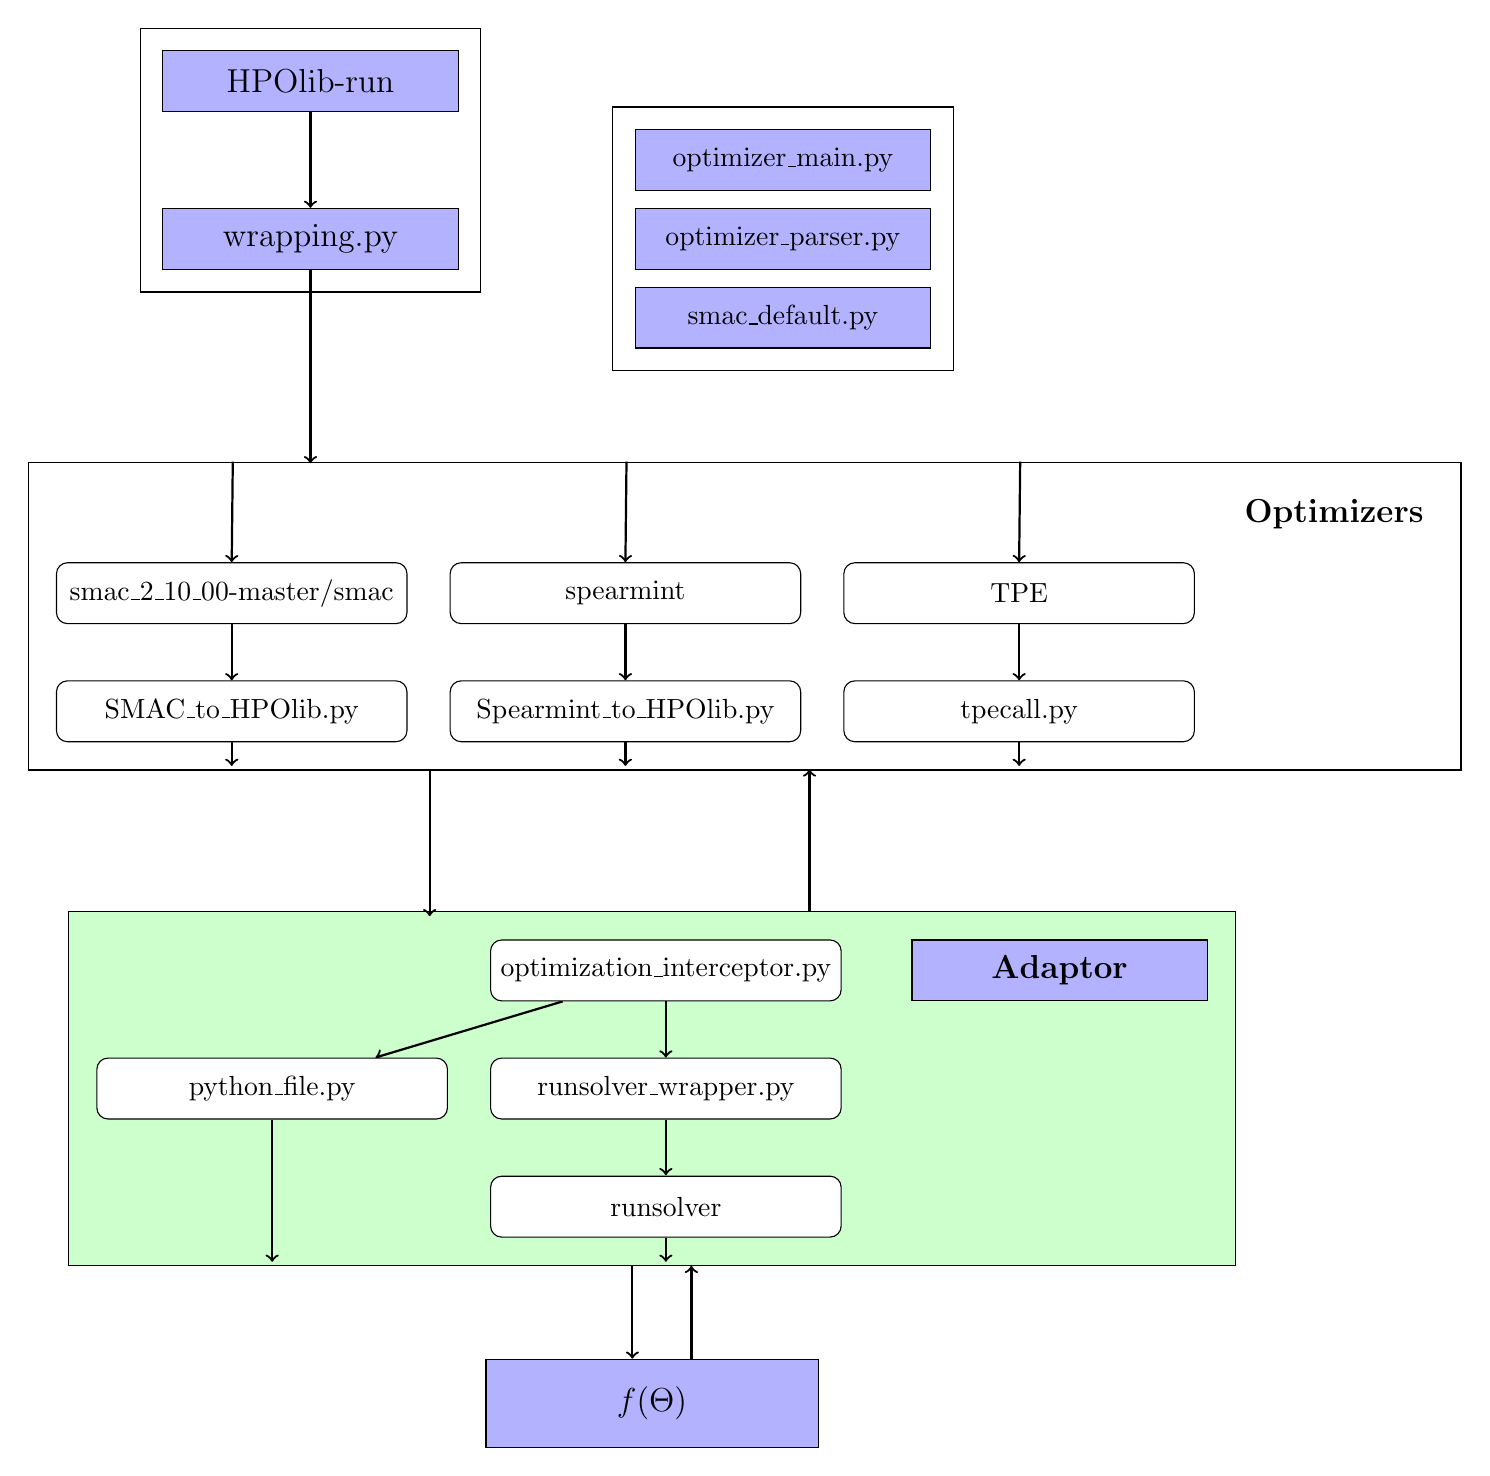
\begin{tikzpicture}[node distance=2cm]

 		\node (HPOlib-run) [core] {\large{HPOlib-run}};
        \node (wrapping) [core, below of=HPOlib-run] {\large{wrapping.py}};
        
		\node [draw=black,inner sep=8pt , fit={(HPOlib-run) (wrapping)}] {};        
        
        \node (optimizer_main) [core, right of=wrapping, node distance=6cm, yshift=1cm] {optimizer\_main.py};
        \node (optimizer_parser) [core, right of=wrapping, node distance=6cm, yshift=0cm] {optimizer\_parser.py};
        \node (smac_default) [core, right of=wrapping, node distance=6cm, yshift=-1cm] {smac\_default.py};

        \node [draw=black,inner sep=8pt , fit={(optimizer_main) (optimizer_parser) (smac_default)}] {};
        
        % Optimizer
        \node (optimizer) [below of=wrapping,node distance=3.5cm, xshift=13cm] {\large{\textbf{Optimizers}}};
       
        \node (SMAC) [data, below of=optimizer, node distance=1cm, xshift=-14cm] {smac\_2\_10\_00-master/smac};
        \node (SMAC_to_HPOlib) [data, below of=SMAC, node distance=1.5cm] {SMAC\_to\_HPOlib.py};

		\node (Spearmint) [data, below of=optimizer, node distance=1cm, xshift=-9cm] {spearmint};
        \node (Spearmint_to_HPOlib) [data, below of=Spearmint, node distance=1.5cm] {Spearmint\_to\_HPOlib.py};
        
        \node (TPE) [data, below of=optimizer, node distance=1cm, xshift= -4cm] {TPE};
        \node (TPEcall) [data, below of=TPE, node distance=1.5cm] {tpecall.py};
                
        
        \node (optimizers) [draw=black,inner sep=10pt ,fit={(SMAC) (SMAC_to_HPOlib) (Spearmint) (Spearmint_to_HPOlib) (TPE) (TPEcall)  (optimizer)}] {};
        
        % Target Function evaluation
    \begin{pgfonlayer} {foreground}
        \node (optimization_interceptor) [data,below of=optimizers,node distance=4.5cm,xshift=-1cm] {optimization\_interceptor.py};
        
        \node (adaptor) [core, right of=optimization_interceptor, node distance=5cm] {\large{\textbf{Adaptor}}};
        
        \node (python_file) [data, below of=optimization_interceptor, node distance=1.5cm,xshift=-5cm] {python\_file.py};
        \node (runsolver_wrapper) [data, right of=python_file, node distance=5cm] {runsolver\_wrapper.py};
        
        
        \node (runsolver) [data, below of=runsolver_wrapper, node distance=1.5cm] {runsolver};
        
	\end{pgfonlayer} {foreground}

	\begin{pgfonlayer} {background}
	
        \node (opt_interceptor)[draw=black,inner sep=10pt, fill=green!20, fit={(optimization_interceptor) (python_file) (runsolver_wrapper) (runsolver) (adaptor)}] {};

	\end{pgfonlayer} {background}
	        
        % Target Function
        \node (function) [core, below of=opt_interceptor, node distance=4cm,inner sep=10pt ] {\large{\textbf{$f(\Theta)$}}};
        
        %Arrows
        
        \draw[myarrow] (HPOlib-run) -- ($(wrapping.north)+(0,0)$);
		\draw[myarrow] (wrapping) -- +(0,-2.85);

		%Optimizers Arrows
		\draw[myarrow] ($(optimizers.north)+(-6.5,-0.0)$) -- ($(SMAC.north)+(0,0)$);
		\draw[myarrow] ($(optimizers.north)+(-1.5,-0.0)$) -- ($(Spearmint.north)+(0,0)$);
		\draw[myarrow] ($(optimizers.north)+(3.5,-0.0)$) -- ($(TPE.north)+(0,0)$);
		
        \draw[myarrow] (SMAC.south) -- ($(SMAC_to_HPOlib.north)+(0,0)$);
        \draw[myarrow] (Spearmint.south) -- ($(Spearmint_to_HPOlib.north)+(0,0)$);
        \draw[myarrow] (TPE.south) -- ($(TPEcall.north)+(0,0)$);

		\draw[myarrow] (SMAC_to_HPOlib.south) -- +(0,-.3);
        \draw[myarrow] (Spearmint_to_HPOlib.south) -- +(0,-.3);
        \draw[myarrow] (TPEcall.south) -- +(0,-.3);
        
        %Optimizers <-> opt_interceptor Arrows
        \draw[myarrow] ($(optimizers.south)+(-4,0)$) -- +(0,-1.85) ;                	
        \draw[myarrow] ($(opt_interceptor.north)+(2,0)$) -- +(0,1.8);

		%opt_interceptor Arrows
		\draw[myarrow] (runsolver_wrapper) -- +(0,-1.1);
		\draw[myarrow] (runsolver) -- +(0,-.7);
		\draw[myarrow] (optimization_interceptor) -- (runsolver_wrapper);
		\draw[myarrow] (optimization_interceptor) -- (python_file);
		\draw[myarrow] (python_file) -- +(0,-2.2);


        %opt_interceptor Arrows
        \draw[myarrow] ($(opt_interceptor.south)-(0.25,0)$) -- ($(function.north)+(-.25,0)$);
        \draw[myarrow] ($(function.north)+(0.5,0)$) -- ($(opt_interceptor.south)-(-0.5,0)$);

\end{tikzpicture}
\end{document}